\section{Extended Experiments and Failure-Directed Diagnostics}

\begin{table*}[t]
  \centering
  \caption{nuScenes-only selective repair and AV2 zero-shot transfer. False repair is measured over all Actors; coverage is
  the accepted fraction. Chamfer is for the repair-or-clean-query output. Leak is the maximum mean prediction shift under a
  paired swap of the other task's input. Each head's nuScenes-calibrated threshold is reused unchanged on AV2.}
  \label{tab:p4-selective}
  \small
  \setlength{\tabcolsep}{4.2pt}
  \begin{tabular}{llrrrrrr}
    \toprule
    Dataset & Head & Repair AUROC $\uparrow$ & Hazard AUROC $\uparrow$ & Coverage $\uparrow$ & False repair $\downarrow$ & Selective CD $\downarrow$ & Max leak $\downarrow$ \\
    \midrule
    nuScenes test & shared & 64.26 & 91.66 & 11.84 & 3.51 & 0.231 & 28.86 \\
    nuScenes test & factorized & \textbf{64.91} & \textbf{98.11} & 3.95 & \textbf{0.44} & 0.246 & \textbf{0.00} \\
    AV2 zero-shot & shared & \textbf{77.97} & 92.89 & 55.21 & \textbf{3.15} & 0.190 & 23.46 \\
    AV2 zero-shot & factorized & 69.96 & \textbf{98.05} & \textbf{75.55} & 8.99 & \textbf{0.182} & \textbf{0.00} \\
    \bottomrule
  \end{tabular}
\end{table*}


\begin{figure*}[t]
  \centering
  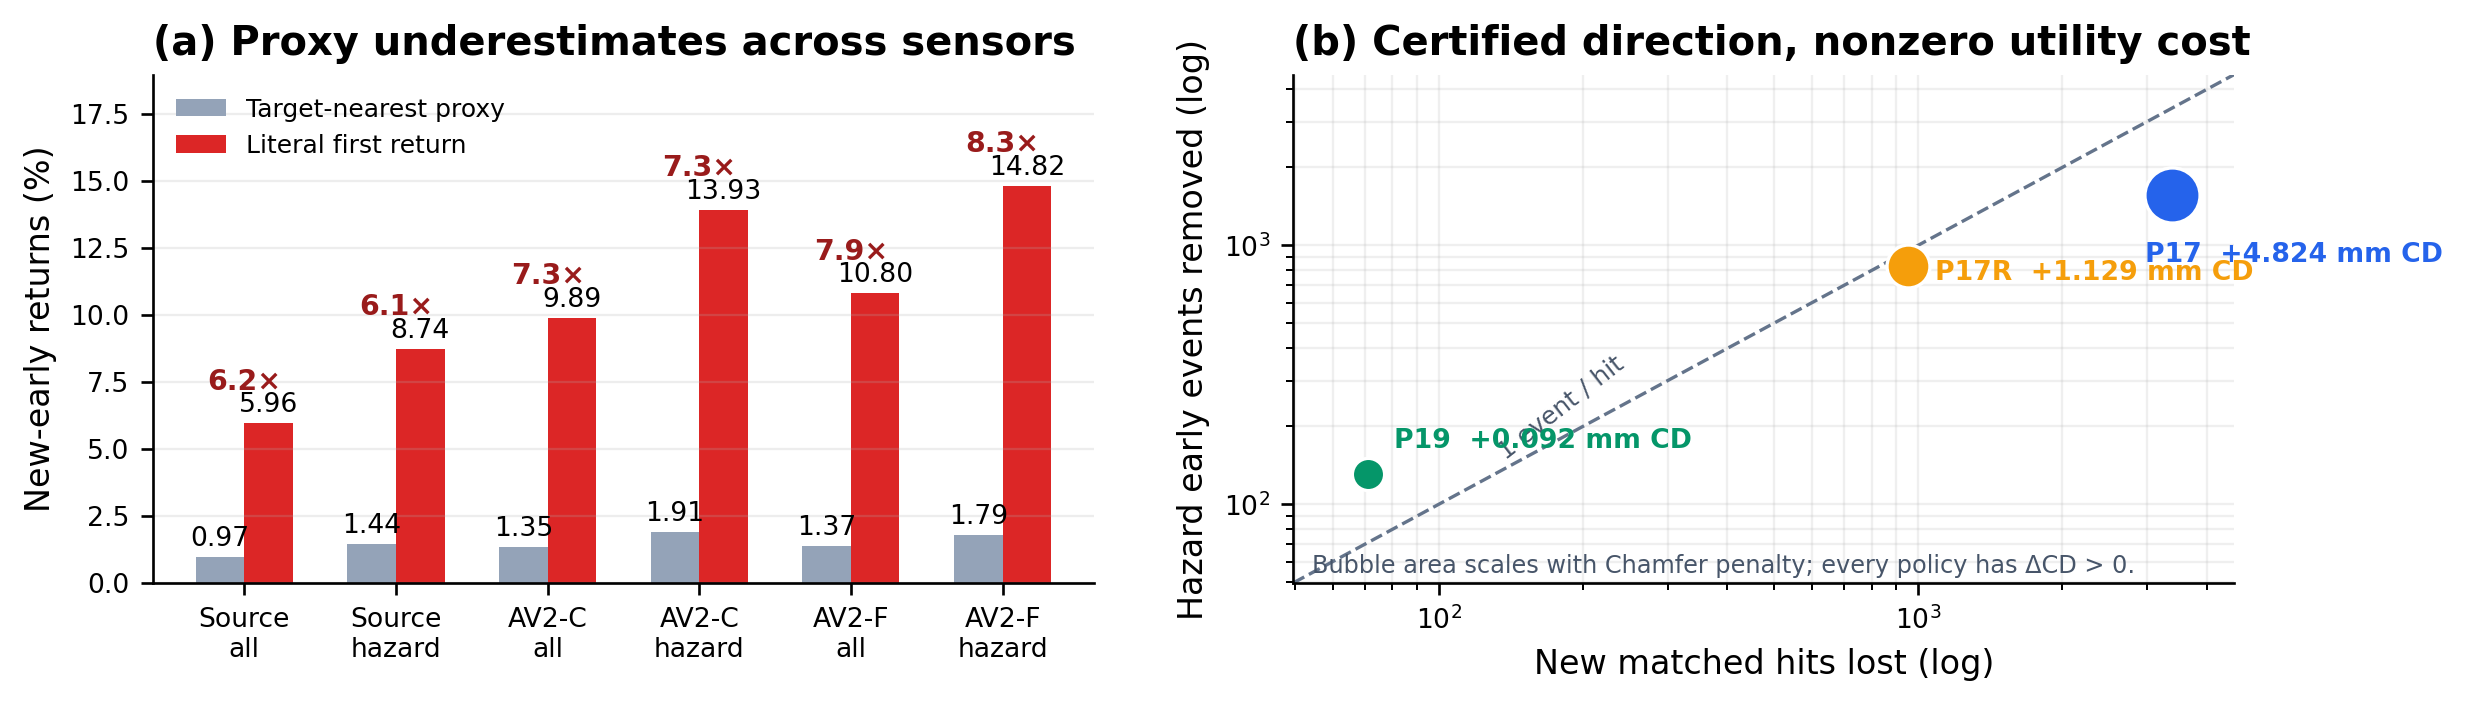
\includegraphics[width=.71\textwidth]{figures/supplement/p21_first_return_boundary.png}\hfill
  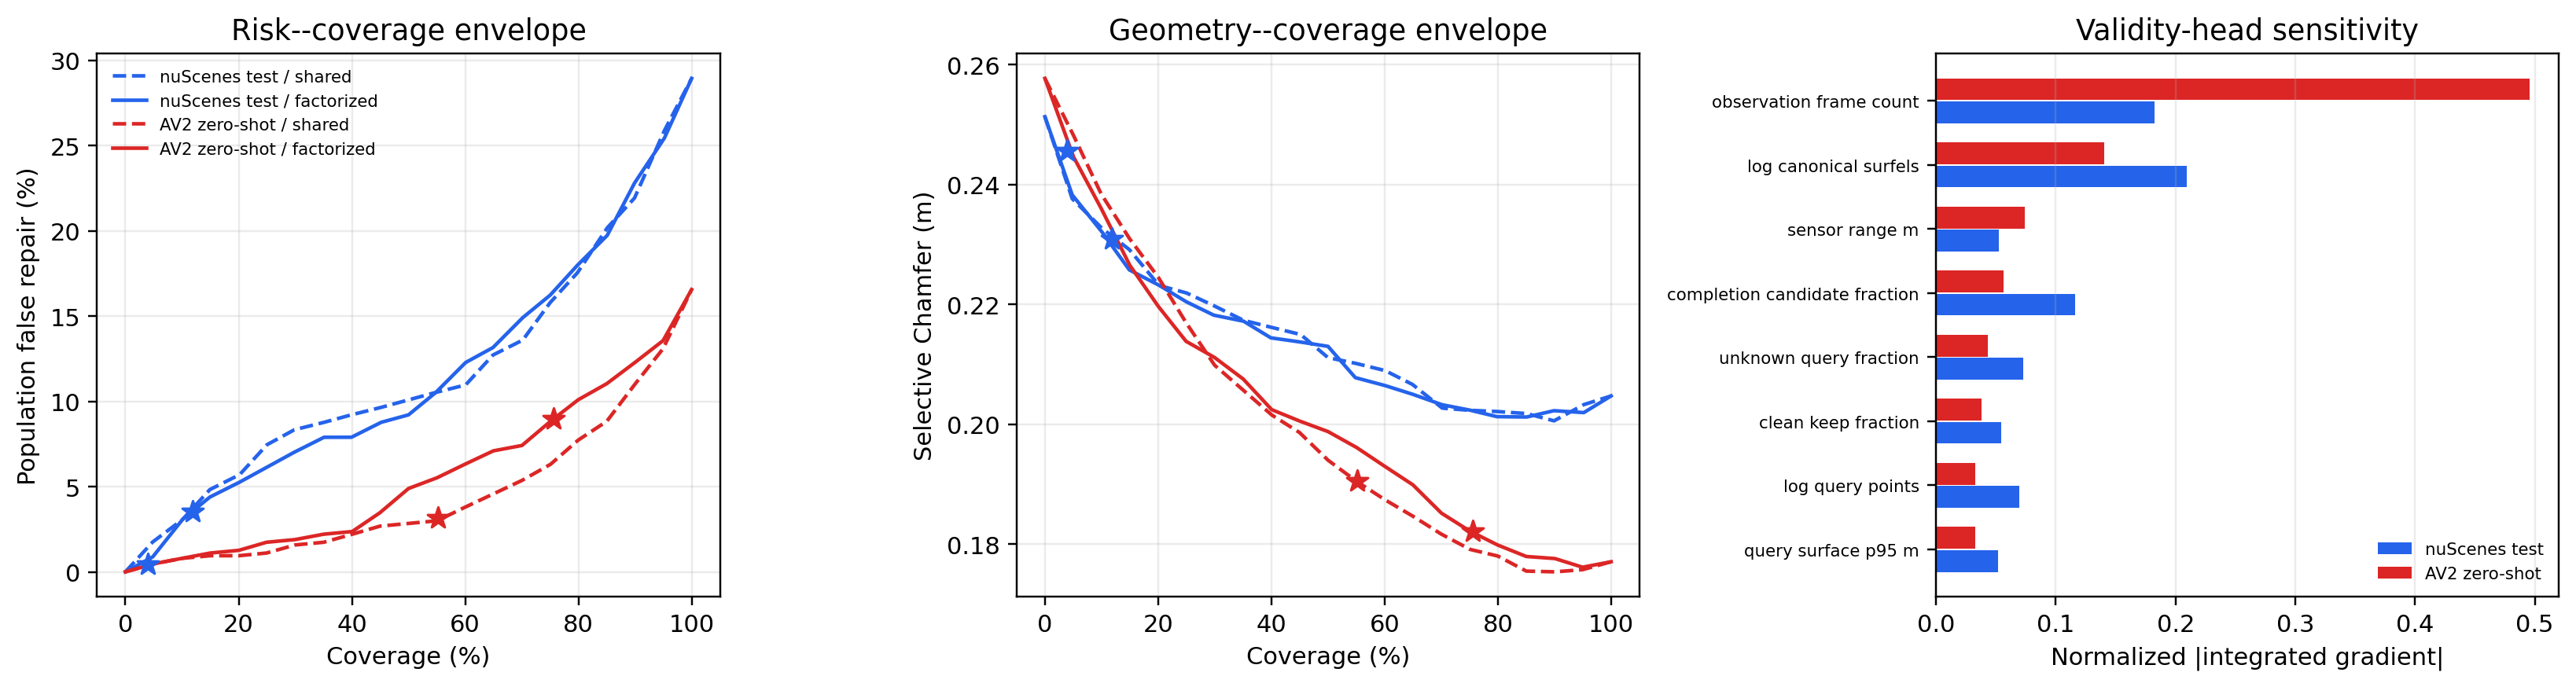
\includegraphics[width=.25\textwidth,trim=700 0 0 0,clip]{figures/p7_interpretable_safety_envelope.png}
  \caption{Physical hard evidence and boundaries. Left: target-nearest proximity undercounts literal first-return exposure on
  source, consumed AV2 (AV2-C), and disjoint exact-once AV2 (AV2-F). Center: deletion certifies non-increasing early returns, but
  every frozen policy loses hits and worsens Chamfer. Right: attribution localizes the AV2 sensor-opportunity shortcut. These are
  measurement, structural-direction, and model-sensitivity results---not collision or road-safety certificates.}
  \label{fig:hard-evidence-boundary}
\end{figure*}

\paragraph{Data and protocol.}
We train and select models only on nuScenes. Argoverse~2 Sensor validation logs form a zero-shot external test. Before reading any method output, we sort the 150 validation UUIDs and select every fifth log, yielding 20 quantitative and 10 qualitative logs. No AV2 fine-tuning, post-hoc calibration, threshold selection, or failed-scene deletion is allowed. Final nuScenes and AV2 cohorts are evaluated exactly once after the method freezes.

\paragraph{Baselines.}
For physical compilation we compare naive reconstruction, a legacy validity filter, V6.7 inward-ray repair, and \method. For factorization we compare a shared encoder, a two-head shared trunk, independent encoders, and paired factorization. Reliability baselines include a scalar confidence, independent horizon classifiers, a continuous marginal density, and the full joint multi-horizon surface.

\paragraph{Metrics.}
Physical metrics include free-space violation, ray termination, point-to-surface error, LiDAR depth consistency, temporal jitter, ghost components, and surface completeness. Hazard preservation reports Actor/ID/lifecycle retention, trajectory and TTC shift, and event-count change. Factorization reports artifact/hazard AUROC and AUPRC, clean-hazard false-artifact rate, paired prediction shift, and cross-probe leakage. Reliability reports log likelihood, integrated Brier score, calibration error, Spearman correlation, monotonic violations, and runtime.

\paragraph{Continuous geometry oracle and learned displacement.}
On train-only Actors, a bounded ray/normal displacement oracle reduces hazardous literal early returns by
\VSevenOneSOneHazardEarlyReduction{} while changing mean Chamfer by \VSevenOneSOneChamferDeltaMm{}\,mm and retaining all
Actor states. This establishes a feasible continuous action space without deleting completion candidates. The fixed M0 residual
model does not reproduce that Pareto point on the \VSevenOneMZeroSelectionActors{}-Actor source selection set. Hazardous early
returns fall by \VSevenOneMZeroHazardEarlyReduction{}, but Chamfer changes by \VSevenOneMZeroChamferDeltaMm{}\,mm and hit
recall by \VSevenOneMZeroHitRecallDeltaPp{} percentage points. It labels \VSevenOneMZeroUnknownFraction{} of completion
candidates unknown, so the apparent ray benefit is principally abstention rather than learned relocation. We therefore
\VSevenOneMZeroVerdict{} M0 under the pre-registered Pareto rule and evaluate the conditionally specified implicit field next.
The field further reduces hazardous early returns by \VSevenOneMOneHazardEarlyReduction{}, but changes Chamfer by
\VSevenOneMOneChamferDeltaMm{}\,mm and hit recall by \VSevenOneMOneHitRecallDeltaPp{} points. It extracts
\VSevenOneMOneFieldPoints{} learned surface points on every selection Actor and therefore degenerates to observed hard anchors.
We \VSevenOneMOneVerdict{} the field, do not tune extraction after selection, and withhold source-final and AV2 claims.

The non-learned B4 evidential TSDF exposes the opposite endpoint on \VSevenOneBFourActors{} selection Actors. It adds
\VSevenOneBFourAddedPoints{} surface points, changes Chamfer by \VSevenOneBFourChamferDeltaMm{}\,mm and hit recall by
\VSevenOneBFourHitRecallDeltaPp{} points, but hazardous early-return reduction is
\VSevenOneBFourHazardEarlyReduction{}---i.e., exposure more than doubles. Table~\ref{tab:v71-continuous-geometry} therefore
shows a two-sided failure boundary rather than a winning learned surface model.

We then correct the training target rather than its deployed output. M5 removes the UNKNOWN action and projects the measured
first-return/surface gradient conflict, passing all five development gates. Directly matching one Gaussian center to one nearest
target point (M6) learns center, tangent-plane, and scale labels but misses the hazardous-ray gate: candidate-bearing Actors have
only 17 completion seeds versus 966 target endpoints at the median. M7 instead performs fixed four-child set expansion. Its
training Chamfer ratio falls from $0.986$ to $0.972$ before physical fine-tuning. On the same
\VSevenOneMFiveDevelopmentActors{} exposed development Actors, it reduces hazardous/all early returns by
\VSevenOneMSevenHazardEarlyReduction{}/\VSevenOneMSevenAllEarlyReduction{}, changes Chamfer by
\VSevenOneMSevenChamferDeltaMm{}\,mm, and increases hit recall by \VSevenOneMSevenHitRecallDeltaPp{} points with complete
Actor and hazard retention. M5 gives \VSevenOneMFiveHazardEarlyReduction{} and \VSevenOneMFiveChamferDeltaMm{}\,mm on this
fold; M6 gives \VSevenOneMSixHazardEarlyReduction{} and is rejected. These are model-development results because the parent
representation previously saw the fold; the frozen AV2 evaluation is reported only after all 20 logs complete.

\begin{table}[t]
\centering
\caption{Frozen V7.1 continuous-geometry evidence. Early is relative hazardous literal first-return reduction (higher is better); CD and hit are changes from each method's query surface. S1 is a train-only oracle. M5--M7 use the same 66-Actor development fold with prior representation exposure and are not external confirmation.}
\label{tab:v71-continuous-geometry}
\resizebox{\columnwidth}{!}{%
\begin{tabular}{lrrrl}
\toprule
Method & Early $\uparrow$ & $\Delta$CD (mm) $\downarrow$ & $\Delta$hit (pp) $\uparrow$ & Decision \\
\midrule
S1 displacement oracle & \VSevenOneSOneHazardEarlyReduction & \VSevenOneSOneChamferDeltaMm & \VSevenOneSOneHitRecallDeltaPp & feasible \\
M0 learned displacement & \VSevenOneMZeroHazardEarlyReduction & \VSevenOneMZeroChamferDeltaMm & \VSevenOneMZeroHitRecallDeltaPp & reject \\
M1 evidential field & \VSevenOneMOneHazardEarlyReduction & \VSevenOneMOneChamferDeltaMm & \VSevenOneMOneHitRecallDeltaPp & reject \\
B4 evidential TSDF & \VSevenOneBFourHazardEarlyReduction & \VSevenOneBFourChamferDeltaMm & \VSevenOneBFourHitRecallDeltaPp & opposite frontier \\
\midrule
M5 PCGrad relocation & \VSevenOneMFiveHazardEarlyReduction & \VSevenOneMFiveChamferDeltaMm & \VSevenOneMFiveHitRecallDeltaPp & dev pass \\
M6 one-to-one GT center & \VSevenOneMSixHazardEarlyReduction & \VSevenOneMSixChamferDeltaMm & \VSevenOneMSixHitRecallDeltaPp & reject \\
M7 GT set child surface & \VSevenOneMSevenHazardEarlyReduction & \VSevenOneMSevenChamferDeltaMm & \VSevenOneMSevenHitRecallDeltaPp & dev pass \\
\bottomrule
\end{tabular}}
\end{table}


\begin{figure*}[t]
\centering
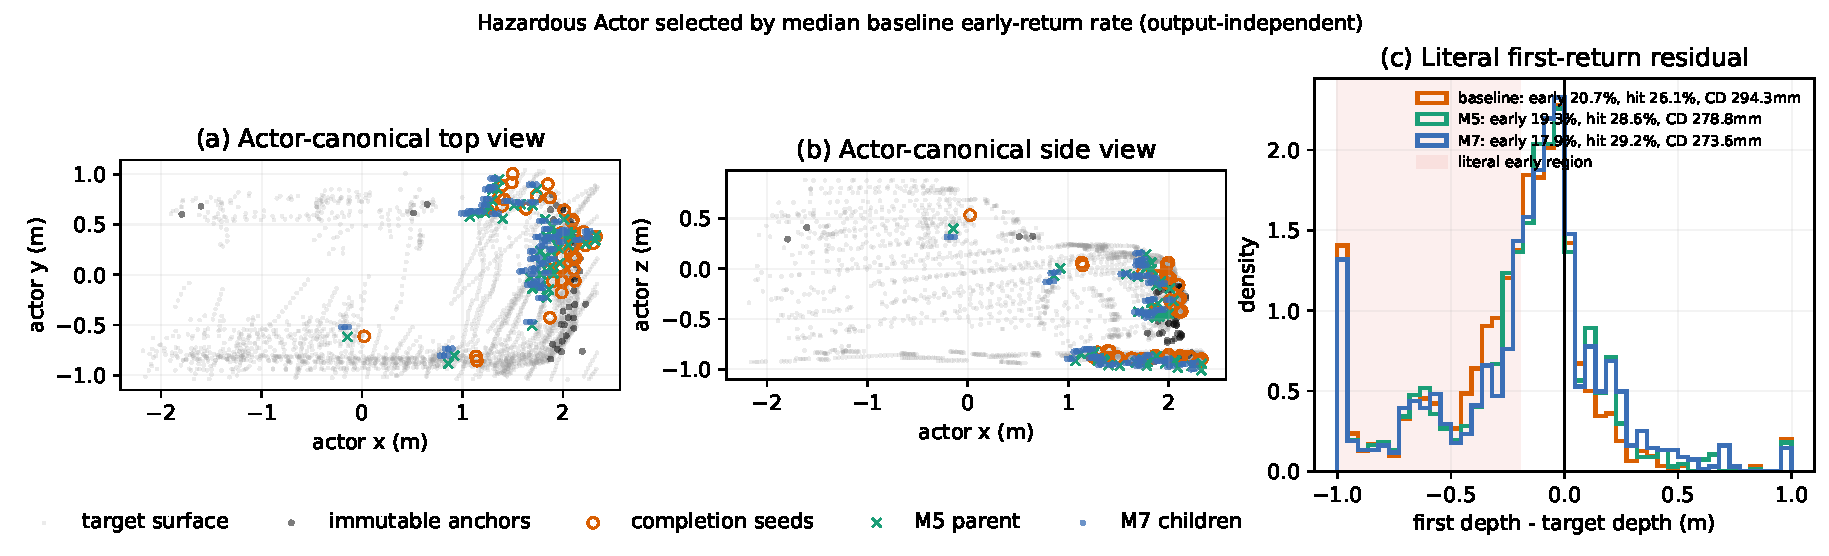
\includegraphics[width=\textwidth]{figures/v71_m7_supervision_native_geometry.pdf}
\caption{Supervision-native geometry on a hazardous development Actor selected by median \emph{baseline} literal early-return
rate, without consulting M7 output. Forty-seven completion seeds expand into 188 child centers while observed anchors remain fixed.
For this output-independent case, baseline/M5/M7 early rates are $20.7/19.3/17.9\%$, hit rates are $26.1/28.6/29.2\%$, and
Chamfer distances are $294.3/278.8/273.6$\,mm. Gray points are held-out GT and never model input.}
\label{fig:v71-m7-geometry}
\end{figure*}

\paragraph{Supervision-native geometry and first-return distribution.}
We next keep every generated surface and supervise the representation itself. Frame-balanced Actor-canonical seed expansion (M8) reduces hazardous early returns by \VSevenOneMEightHazardEarlyReduction{}, changes Chamfer by \VSevenOneMEightChamferDeltaMm{}\,mm, and changes hit recall by \VSevenOneMEightHitRecallDeltaPp{} points. Analytic and implicit support variants then expose complementary failures (Table~\ref{tab:v71-query-representations}): compact support suppresses early returns but misses the surface, whereas an unconstrained direct field restores hits but creates earlier sign changes. Non-negative survival density restores monotonicity but accumulates diffuse pre-hit opacity.

The categorical model (M18) is the only frozen development candidate satisfying all seven point/ray gates. Relative to M8 it reduces hazardous/all early returns by \VSevenOneMEighteenHazardEarlyReduction{}/\VSevenOneMEighteenAllEarlyReduction{} and raises hazardous/all hit recall by \VSevenOneMEighteenHazardHitDeltaPp{}/\VSevenOneMEighteenAllHitDeltaPp{} points, with 100\% observable rays. The clear subset remains negative (early \VSevenOneMEighteenClearEarlyReduction{}, hit \VSevenOneMEighteenClearHitDeltaPp{} points), so this is not a uniform dominance or safety result. The fold was exposed to the M8 predecessor; no partial external metric is used for model choice, and the eventual frozen M39 AV2 test rejects transfer.

\begin{table}[t]
\centering
\caption{Frozen query-representation ablation on the exposed nuScenes development fold. Early is hazardous relative reduction and hit is hazardous recall change, both versus M8. Only M18 satisfies the pre-registered early and hit gates; no row is an external result.}
\label{tab:v71-query-representations}
\resizebox{\columnwidth}{!}{%
\begin{tabular}{llrrr}
\toprule
ID & Query representation & Early $\uparrow$ & $\Delta$hit (pp) $\uparrow$ & Obs. (\%) \\
\midrule
M13 & blended local planes & -76.68\% & -10.57 & 95.90 \\
M14 & compact radial patches & +69.12\% & -24.15 & 39.89 \\
M15 & one-sided surface cells & +35.11\% & -13.54 & 60.41 \\
M16 & direct signed queries & -11.98\% & +2.07 & 93.51 \\
M17 & monotone survival density & +26.52\% & -26.14 & 96.18 \\
M18 & categorical first return & \textbf{+7.63\%} & \textbf{+6.60} & \textbf{100.0} \\
\bottomrule
\end{tabular}}
\end{table}


Joint training exposes a stricter identifiability boundary (Table~\ref{tab:v71-joint-energy}). M19 lets the learned field update completed children: Chamfer improves by $2.42$\,mm versus M8, but the point-surface hazardous early direction reverses from a $5.12\%$ reduction to a $4.10\%$ increase. Its apparently larger field-over-point gain therefore compensates for a degraded reference; absolute field early rate is slightly worse than M18. M20 removes the field decoder, yet predicted scale expands from $0.162$ to $0.313$\,m on average. Its categorical NLL falls while point early returns and the analytic energy both worsen relative to their M8 initialization. We reject both fine-tuning paths.

The diagnostic nevertheless identifies a simpler candidate: frozen M8 geometry followed by the same decoder-free energy gives $17.42\%$ hazardous early rate and $62.07\%$ hit recall, without modifying a Gaussian after its native-3D supervision. This M21 row is selected on the exposed development fold, so it is not an independent result. We freeze its representation and the existing 20-log AV2 cohort before reading any partial quality; the later M39 external run rejects zero-shot transfer without target adaptation.

\begin{table}[t]
\centering
\caption{Failure-directed coupling diagnostic on the exposed nuScenes development fold. Point early is hazardous relative reduction versus the original completion (negative is worse). Energy columns are absolute hazardous early rate and hit recall. M21 reuses frozen M8 geometry and was selected by this diagnostic; it is not an external result.}
\label{tab:v71-joint-energy}
\resizebox{\columnwidth}{!}{%
\begin{tabular}{llrrr}
\toprule
ID & Representation & Point early $\uparrow$ & Energy early $\downarrow$ & Energy hit $\uparrow$ \\
\midrule
M18 & frozen M8 + learned field & $+5.12\%$ & $24.36\%$ & $57.24\%$ \\
M19 & joint geometry + learned field & $-4.10\%$ & $24.43\%$ & $58.47\%$ \\
M20 & joint geometry + analytic energy & $-3.25\%$ & $19.88\%$ & $57.33\%$ \\
M21 & frozen M8 + analytic energy & $+5.12\%$ & $17.42\%$ & $62.07\%$ \\
\bottomrule
\end{tabular}}
\end{table}


\paragraph{Zero-shot Actor-local surface evidence.}
Following the dynamic-Actor canonicalization boundary used by NeuRAD~\cite{tonderski2024neurad}, we transform ego-frame AV2
LiDAR points inside each annotated cuboid into its Actor frame. Unlike appearance-oriented seed initialization, we never mirror
points: every collision surfel must retain sensor and temporal support. We fuse two of every three frames at $0.12$\,m and reserve
the remaining frames as unseen target geometry. Across \PoneActors{} Actors and \PoneSurfels{} stable surfels, fusion reduces the
mean target-to-surface distance from \PoneSingleDistance{}\,m to \PoneFusedDistance{}\,m and raises recall at $0.20$\,m from
\PoneSingleRecall{}\% to \PoneFusedRecall{}\% (Table~\ref{tab:p1-av2-surface}).

The paired corruption atlas contains clean, observed-free ghost, duplicate-shell, temporal-flicker, and supported-hole probes
without changing Actor identity, trajectory, size, or hazard. It yields \PoneArtifactRecall{}\% artifact recall,
\PoneHazardFA{}\% clean-hazard false-artifact rate, and \PoneActorRetention{}\% Actor/hazard retention. These perfect paired
scores verify the deterministic compiler contract and input separation; they are not reported as natural-artifact generalization.

\begin{table}[t]
    \centering
    \small
    \setlength{\tabcolsep}{4pt}
    \begin{tabular}{lcc}
        \toprule
        AV2 Actor surface & Dist. (m) $\downarrow$ & Recall (\%) $\uparrow$ \\
        \midrule
        Single observed frame & \PoneSingleDistance & \PoneSingleRecall \\
        Multi-frame canonical surfels & \textbf{\PoneFusedDistance} & \textbf{\PoneFusedRecall} \\
        \bottomrule
    \end{tabular}
    \caption{Zero-shot held-out LiDAR support on the frozen 20-log AV2 quantitative cohort
    (\PoneActors{} Actors, including \PoneHazardActors{} hazardous Actors). The comparison uses real sensor points;
    paired synthetic corruptions are evaluated separately as a compiler contract.}
    \label{tab:p1-av2-surface}
\end{table}


\paragraph{Four-action physical compilation.}
We next freeze one single-frame query per Actor and reserve all later held-out frames as target-only geometry. The compiler
reads only the build surface and query evidence. A nearest-canonical projection initially reduces Chamfer to
\PtwoChamferAfter{}\,m, but ray-specific evaluation reveals \PthreeFreeNearest{}\% early terminations in the paired observed-free
interval. Our final operator is ray-certified: a primitive with direct LiDAR provenance projects to its matched observed
termination; without one it becomes \textsc{unknown}. Across \PtwoActors{} quantitative Actors (\PtwoHazardActors{} hazardous),
this reduces paired free-space violations from \PthreeFreeBefore{}\% to \PthreeFreeAfter{}\%, target depth error from
\PthreeDepthBefore{}\,m to \PthreeDepthAfter{}\,m, and Chamfer from \PtwoChamferBefore{}\,m to \PthreeChamferAfter{}\,m,
while raising ray-termination consistency from \PthreeRayBefore{}\% to \PthreeRayAfter{}\% (Table~\ref{tab:p2-four-action}).
Actor identity, trajectory, extent, and hazard labels are retained for \PtwoActorRetention{}\% of Actors. The zero free-space
rate is a paired contract result; depth, ray termination, and Chamfer use independent target-only LiDAR.

\begin{table}[t]
    \centering
    \small
    \setlength{\tabcolsep}{3.5pt}
    \begin{tabular}{lccc}
        \toprule
        Surface & Free (\%) $\downarrow$ & Recall (\%) $\uparrow$ & CD (m) $\downarrow$ \\
        \midrule
        Single-frame input & \PthreeFreeBefore & \PtwoRecallBefore & \PtwoChamferBefore \\
        Nearest canonical & \PthreeFreeNearest & \textbf{\PtwoRecallAfter} & \textbf{\PtwoChamferAfter} \\
        Ray-certified & \textbf{\PthreeFreeAfter} & \PthreeRecallAfter & \PthreeChamferAfter \\
        \bottomrule
    \end{tabular}
    \caption{Frozen zero-shot AV2 quantitative result. Nearest-surface projection fits geometry best but violates matched-ray
    free space; ray-certified projection accepts a small Chamfer cost. Later held-out frames are target-only.}
    \label{tab:p2-four-action}
\end{table}


\paragraph{Frozen camera evidence and an exposed boundary.}
We project each pre-registered qualitative Actor back into synchronized AV2 ring-camera frames using the official calibration
and motion compensation. Camera identity maximizes only the number of visible query LiDAR returns, with a fixed camera-order
tie break; RGB is decoded afterward and every case is retained. All \PthreeBCases{} cases have calibrated RGB, sparse depth,
four-action, and before/after video evidence; the median/minimum visible query counts are
\PthreeBMedianVisible{}/\PthreeBMinimumVisible{} (Fig.~\ref{fig:p3b-camera}). Importantly, the frozen set exposes a limit:
although mean Chamfer improves, \PthreeActorWorse{}\% of all 634 Actors worsen individually. Thus P3 establishes aggregate
zero-shot geometry, not a per-Actor repair certificate; this motivates a selective ``repair or abstain'' validity head trained
and calibrated only on nuScenes.

\paragraph{Visibility-conditioned physical evidence.}
We further partition target-only LiDAR evidence with a target-nearest proximity operator into early, matched hit, late, and unmatched; reverse
surface evidence is supported, contradicted by observed free space, occluded, or off-ray unknown. Unknown is never counted as
free. On all \PthreeCActors{} Actors, query-to-compiled hit recall rises from \PthreeCQueryHit{}\% to
\PthreeCCompiledHit{}\%, early termination falls from \PthreeCQueryEarly{}\% to \PthreeCCompiledEarly{}\%, and visible-surface
precision rises from \PthreeCQueryPrecision{}\% to \PthreeCCompiledPrecision{}\% (F-score
\PthreeCQueryFscore{}$\rightarrow$\PthreeCCompiledFscore{}). Yet only \PthreeCNonnewActors{}\% of Actors add no visible
violation. An independent 20-log read reproduces hit
\PthreeFreshQueryHit{}$\rightarrow$\PthreeFreshCompiledHit{}\%, early
\PthreeFreshQueryEarly{}$\rightarrow$\PthreeFreshCompiledEarly{}\%, and F-score
\PthreeFreshQueryFscore{}$\rightarrow$\PthreeFreshCompiledFscore{}, while only \PthreeFreshNonnewActors{}\% add no visible
violation and \PthreeFreshChamferWorse{}\% worsen in Chamfer. Provenance attribution explains the trade-off: completion supplies \PthreeDCompletionNewEarly{}\% of new early rays
but \PthreeDCompletionGain{} new hits per such ray, while only \PthreeDCompletionContradiction{}\% of contradicted output points
come from completion. We therefore retain the net \PthreeDNetEarlyReduction{}-ray reduction, reject a universal certificate,
and route Actor-level authority through abstention rather than delete completion. These frozen values localize errors around each
target return; they are not literal first-return rates, which are audited below over every candidate surface point in the beam tube.

\paragraph{nuScenes-to-AV2 selective factorization.}
The strict multi-frame surface contract yields 29/56/\PfourNuActors{} Actors for nuScenes train/calibration/test; we retain the
small training set rather than loosen admissibility. On nuScenes test, factorization is non-inferior to the shared head for
repairability (\PfourNuFactorRepairAUROC{} vs.\ \PfourNuSharedRepairAUROC{} AUROC) and raises hazard AUROC from
\PfourNuSharedHazardAUROC{} to \PfourNuFactorHazardAUROC{}, while maximum paired cross-input shift falls from
\PfourSharedLeakage{}\% to \PfourFactorLeakage{}\%. The conservative threshold covers \PfourNuFactorCoverage{}\% with
\PfourNuFactorFalseRepair{}\% population false repairs.

Without AV2 fitting, the same selector covers \PfourAVFactorCoverage{}\% of \PfourAVActors{} Actors and reduces false repair
from \PfourAVAlwaysFailure{}\% under always-repair to \PfourAVFactorFalseRepair{}\%. Clean-query/always/selective Chamfer is
\PfourAVQueryChamfer{}/\PfourAVAlwaysChamfer{}/\PfourAVSelectiveChamfer{}\,m. Thus abstention costs only $5$\,mm mean Chamfer
relative to always-repair while nearly halving false repairs. Hazard AUROC is \PfourAVFactorHazardAUROC{}, hazard coverage is
\PfourAVHazardCoverage{}\%, and factorized cross-input shift remains zero. However, coverage changes from
\PfourCalibrationCoverage{}\% on nuScenes calibration to \PfourAVFactorCoverage{}\% on AV2; Table~\ref{tab:p4-selective}
therefore supports empirical transfer, not a cross-domain conformal guarantee.

\paragraph{Interpretable safety envelope.}
We retain the model, standardizer, thresholds, and all Actor rows and evaluate 21 fixed coverage levels without refitting or
recalibration. The factorized score shifts from mean/median $.761/.945$ on nuScenes calibration to $.978/.999992$ on AV2
(Wasserstein $.217$, KS $.704$), explaining the operating-point coverage jump. Integrated Gradients~\cite{sundararajan2017axiomatic}
relative to the nuScenes-training mean attributes 18.25\% of absolute validity sensitivity to observation-frame count on
nuScenes test but 49.53\% on AV2 (Fig.~\ref{fig:hard-evidence-boundary}, right). The complete fixed-threshold risk--coverage and
geometry--coverage curves remain in the supplement. Structural cross-input derivatives remain exactly zero: task factorization
prevents hazard leakage, but does not make validity inputs sensor invariant. We therefore preserve the empirical P4 result while
rejecting the stronger interpretation of a domain-invariant selector.

We then propagate fixed $0.10$ nuScenes-training-standard-deviation feature boxes through the frozen validity MLP in FP64.
Only \PsevenCTestCertified{}\% of nominal nuScenes-test selections are robust to the full box, versus
\PsevenCAVCertified{}\% on consumed AV2. Yet \PsevenCAVStableFalse{}\% of those AV2 robust selections are target false repairs:
local threshold invariance can stably preserve a domain-shifted error. Sensor-opportunity perturbations create mean logit widths
of \PsevenCTestOpportunityWidth{}/\PsevenCAVOpportunityWidth{} on nuScenes/AV2, and query-point count is the largest
single-feature interval source for \PsevenCTestQueryTop{}/\PsevenCAVQueryTop{}\% of Actors. This actor-level certificate makes
the shortcut inspectable, while explicitly separating network stability from repair correctness.

\paragraph{Fresh exact-once selector boundary.}
Before this read, we exclude every P4 train/calibration/test scene and freeze 20 of the remaining 106 locally available scenes
by equally spaced official scene index. The 20 scenes yield \PeightActors{} Actors and are read once, with no replacement or
model/threshold update. Motivated by source-only LiDAR sparsity consistency~\cite{kim2023dglss}, a pre-frozen candidate increases
coverage from \PeightPfourCoverage{}\% to \PeightCandidateCoverage{}\% and improves selective Chamfer from
\PeightPfourChamfer{} to \PeightCandidateChamfer{}\,m. It nevertheless lowers repair AUROC from
\PeightPfourRepairAUROC{} to \PeightCandidateRepairAUROC{} and fails the pre-registered 2-point non-inferiority margin
(Table~\ref{tab:p4-selective}). A descriptive common-coverage audit follows the selective-classification AURC formulation
of Zhou \etal~\cite{zhou2025aurc}: candidate/P4 AURC is \PeightCandidateAURC{}/\PeightPfourAURC{} (lower is better), confirming
global ranking loss rather than only threshold mismatch. We retain the P4 selector; the recovery remains a negative ablation.

On \PsixFreshActors{} exact-once AV2 Actors, the order reverses: candidate/P4 AUROC is
\PsixFreshCandidateRepairAUROC{}/\PsixFreshPfourRepairAUROC{} and Chamfer
\PsixFreshCandidateChamfer{}/\PsixFreshPfourChamfer{}\,m, but false repair is
\PsixFreshCandidateFalseRepair{}/\PsixFreshPfourFalseRepair{}\%. External gates pass, yet this source/external reversal is
cohort-dependent rather than universal; P4 remains primary.

\paragraph{Physical authority is not a visibility certificate.}
We exact-join the same \PtenActors{} fresh AV2 Actors to the independently frozen bidirectional visibility audit, without
changing either score or threshold. P4 selects \PtenPfourCoverage{}\%; its Chamfer-worsening rate falls from
\PtenAlwaysChamferWorse{}\% under always-repair to \PtenSelectedChamferWorse{}\%. Selected visible-failure risk changes only
from \PtenAlwaysVisibleRisk{}\% to \PtenSelectedVisibleRisk{}\%, and its one-sided 95\% Wilson upper bound
\PtenSelectedVisibleUpper{}\% remains above the always-repair point risk. Safe-visible AUROC is \PtenVisibleSafeAUROC{}, and
abstention captures \PtenVisibleCapture{}\% of visible failures. Thus P4 controls its Chamfer target but does not
confidence-separate visibility risk. Requiring no \textsc{complete} output and conjoining with P4 lowers visible failure to
\PelevenDualVisibleRisk{}\% at \PelevenDualCoverage{}\% coverage, but Chamfer worsening rises to
\PelevenDualChamferWorse{}\% and hazard coverage collapses to \PelevenDualHazardCoverage{}\%; observed provenance is therefore
visibility evidence, not jointly valid repair authority.

A dedicated nuScenes-only visibility head confirms this mismatch rather than solving it. Safe-visible AUROC is
\PtwelveSourceSafeAUROC{} on source test and \PtwelveExternalSafeAUROC{} on AV2. Visibility-only selection reaches
\PtwelveVisibilityRisk{}\% AV2 visible risk at \PtwelveVisibilityCoverage{}\% coverage; conjunction with P4 reaches
\PtwelveDualVisibleRisk{}\% (95\% upper \PtwelveDualVisibleUpper{}\%) at \PtwelveDualCoverage{}\% coverage. Yet dual
Chamfer-worsening is \PtwelveDualChamferWorse{}\% and hazard coverage is \PtwelveDualHazardCoverage{}\%. We reject the head:
low target-specific risk obtained by losing geometry and hazardous Actors is not a safety authority.

The complete defer-to-query system preserves \PthirteenActorRetention{}\% of Actors and separates conditional risk from
population utility. P4 has \PthirteenPfourPopulationVisible{}\% population introduced-visible failure with
\PthirteenPfourGain{}\,m composite Chamfer gain; P6-C has \PthirteenPsixPopulationVisible{}\% and
\PthirteenPsixGain{}\,m, remaining an AV2-only frontier point because its fresh-nuScenes ranking reverses. P4-and-visibility
has only \PthirteenDualPopulationVisible{}\% introduced failure but \PthirteenDualGain{}\,m gain. In contrast, the provenance
policy has \PthirteenProvenancePopulationVisible{}\% introduced failure and \PthirteenProvenanceGain{}\,m gain, so query-only
strictly dominates it. Low selected risk alone therefore does not establish fallback-system utility.

Exact stratification exposes where this utility is obtained. Hazardous Actors are \PfourteenHazardActorShare{}\% of the cohort;
P4 selected visible risk is \PfourteenPfourHazardRisk{}\%/\PfourteenPfourClearRisk{}\% on hazardous/clear Actors versus
\PfourteenAlwaysHazardRisk{}\%/\PfourteenAlwaysClearRisk{}\% under always-repair. Only
\PfourteenPfourHazardFailureReduction{} of its 48 removed failures are hazardous, yet they carry
\PfourteenPfourHazardFailureShare{}\% of introduced failures and \PfourteenPfourHazardGainShare{}\% of gain. Fresh
target-nearest action attribution localizes the mismatch: hazardous/clear proxy new-early rates are
\PfifteenHazardNewEarlyRate{}\%/\PfifteenClearNewEarlyRate{}\% (\PfifteenHazardClearRatio{}$\times$); COMPLETE causes
\PfifteenCompleteNewEarlyShare{}\% of new early returns and \PfifteenCompleteNewHitShare{}\% of new hits, whereas KEEP causes
\PfifteenKeepContradictionShare{}\% of surface contradictions. P4's hazardous rate is \PfifteenPfourHazardNewEarlyRate{}\%
(\PfifteenPfourHazardVsAlways{}$\times$ always), and P6-C is \PfifteenPsixHazardVsAlways{}$\times$. State preservation
therefore does not imply hazard-stratum risk reduction or suppression of its completion-driven mechanism.

\paragraph{Literal first-return correction and safety--surface boundary.}
The preceding frozen action audit uses the target-nearest point as a proximity attribution. Following raw-ray occupancy
evaluation~\cite{kalble2024accurate}, we separately re-audit fixed source and consumed AV2 surfaces with Eq.~\ref{eq:first-return}. The
source total/hazard proxy rates \PtwentyLegacyTotalEarly{}/\PtwentyLegacyHazardEarly{}\% rise to
\PtwentyTrueTotalEarly{}/\PtwentyTrueHazardEarly{}\%. P17/P17R/P19 reduce hazard exposure to
\PtwentyPseventeenHazardEarly{}/\PtwentyPseventeenRHazardEarly{}/\PtwentyPnineteenHazardEarly{}\%, but each worsens Chamfer.
Thus the certified early direction has nonzero surface cost.

Consumed AV2 first shows hazard exposure \PtwentytwoProxyHazardEarly{}$\rightarrow$\PtwentytwoTrueHazardEarly{}\%
(\PtwentytwoHazardRatio{}$\times$). A disjoint exact-once \PtwentythreeLogs{}-log read then independently confirms all/hazard
\PtwentythreeProxyTotalEarly{}/\PtwentythreeProxyHazardEarly{}$\rightarrow$
\PtwentythreeTrueTotalEarly{}/\PtwentythreeTrueHazardEarly{}\% (\PtwentythreeTotalRatio{}/\PtwentythreeHazardRatio{}$\times$).
All \PtwentythreeTrueNewEarly{} fresh literal new-early rays are \textsc{complete}; completion supplies
\PtwentythreeCompleteNewHitShare{}\% of \PtwentythreeTrueNewHits{} new hits, only \PtwentythreeHitEarlyRatio{} hits/early.
Figure~\ref{fig:hard-evidence-boundary} (left and center) visualizes both findings. They transfer metric failure and provenance,
not model, policy, collision, or road-safety validity.

\paragraph{Frozen continuous and joint reliability.}
We inherit the V6.7 reliability objects without V7 refitting. On \PrelMarginalFreshLogs{} previously unread nuScenes logs,
the five-component log-cost density reduces mean integrated Brier and marginal calibration error by
\PrelMarginalBrierGain{}\% and \PrelMarginalCalibGain{}\% relative to the frozen monotone-CDF control. A conditional
four-horizon copula improves joint-event Brier by \PrelJointDevBrierGain{}\% on source-held-out trajectories and by
\PrelJointFreshBrierGain{}\% on an independently frozen \PrelJointFreshLogs{}-log cohort; calibration-error reductions are
\PrelJointDevCalibGain{}\% and \PrelJointFreshCalibGain{}\% (Table~\ref{tab:c3-reliability}). The downstream P346 authority
reaches \PrelAuthorityFreshCoverage{}\% q90 coverage at \PrelAuthorityFreshUnsafe{}\% unsafe rate on that consumed fresh
cohort, but source held-out-horizon risk rises to \PrelAuthorityHeldoutUnsafe{}\%. We therefore treat density, dependence,
and task authority as separate inherited evidence, not as a V7 repair effect or a formal cross-domain calibration claim.

\begin{table}[t]
  \centering
  \caption{Frozen V6.7 reliability evidence inherited without V7 refitting. P183 has \PrelMarginalFreshLogs{} fresh logs;
  source held-out has \PrelJointDevTrajectories{} trajectories; P201 has \PrelJointFreshTrajectories{} trajectories from
  \PrelJointFreshLogs{} fresh logs. $\Delta$B/$\Delta$E are Brier/calibration-error reductions. P346 reuses P201 and remains
  development evidence.}
  \label{tab:c3-reliability}
  \scriptsize
  \setlength{\tabcolsep}{2.1pt}
  \begin{tabular}{llrrr}
    \toprule
    Object & Split & $\Delta$B $\uparrow$ & $\Delta$E $\uparrow$ & cov./unsafe $\uparrow\!\downarrow$ \\
    \midrule
    density & P183 fresh & \PrelMarginalBrierGain{} & \PrelMarginalCalibGain{} & -- \\
    joint & source held-out & \PrelJointDevBrierGain{} & \PrelJointDevCalibGain{} & -- \\
    joint & P201 fresh & \PrelJointFreshBrierGain{} & \PrelJointFreshCalibGain{} & -- \\
    P346 & P201 reused & -- & -- & \PrelAuthorityFreshCoverage{}/\PrelAuthorityFreshUnsafe{} \\
    P346 & source held-out $H$ & -- & -- & \PrelAuthorityHeldoutCoverage{}/\PrelAuthorityHeldoutUnsafe{} \\
    \bottomrule
  \end{tabular}
\end{table}


\begin{table}[t]
  \centering
  \caption{Frozen physical--trajectory interface on exact-match nuScenes test Actors. Cost and error are row-level 90th
  percentiles over retained V6.7 outcomes; FS/flip gives event counts. Physical selection is not trajectory authority.}
  \label{tab:p5-dual-authority}
  \small
  \setlength{\tabcolsep}{3.6pt}
  \begin{tabular}{lrrrr}
    \toprule
    P4 group & Actors & q90 cost $\downarrow$ & q90 error $\downarrow$ & FS / flip $\downarrow$ \\
    \midrule
    selected & 5 & 0.283 & 1.577 & 0 / 0 \\
    abstained & 83 & 0.102 & 0.693 & 7 / 47 \\
    geometric harm & 23 & 0.076 & 0.543 & 0 / 4 \\
    \bottomrule
  \end{tabular}
\end{table}


\paragraph{Physical repair is not trajectory authority.}
We exact-join P4 identities to retained V6.7 multi-horizon outcome rows through the official nuScenes scene order and
DriveStudio instance tokens. Only 5 P4-train Actors from two scenes align, so we reject joint fitting rather than recycle
calibration/test Actors. The frozen descriptive audit instead contains \PfiveActors{} test Actors and 39,285 rows
(Table~\ref{tab:p5-dual-authority}). P4 selects \PfiveSelectedActors{} Actors and abstains on all \PfiveHarmActors{} whose
compiled Chamfer is worse than the query; selected-and-harmful is therefore zero. Its \PfiveSelectedRows{} selected rows contain
no false-safe or decision-flip events. Nevertheless, selected q90 motion error is \PfiveSelectedQError{}\,m versus
\PfiveAbstainedQError{}\,m for abstained Actors (\PfiveErrorRatio{}$\times$), reaching \PfiveThreeSecondQError{}\,m at 3\,s.
The physical gate protects representation quality but cannot replace the downstream reliability authority. These are retained
source outcomes, not a causal effect of repair or an execution of the reliability model.

We also stress the analytic geometry-to-cost bound on \PsevenBRows{} retained profiles under \PsevenBShifts{} fixed
$\pm0.05/0.10/0.20$\,m shifts. FP64 evaluation has zero violations. At $-0.20$\,m, full-source mean/q99 absolute cost shift is
\PsevenBMeanShift{}/\PsevenBQShift{}, while only \PsevenBSignCross{}\% of rows cross signed clearance. P4-selected versus
abstained mean shift is \PsevenBSelectedShift{}/\PsevenBAbstainedShift{} (\PsevenBStabilityRatio{}$\times$ more stable) with
no selected crossings. Selected Actors can therefore be motion-difficult yet geometrically stable, further separating the three
axes of repairability, geometry sensitivity, and trajectory uncertainty.

\begin{table}[t]
  \centering
  \caption{Retained-source $2\times2$ composition on 88 exact P5 Actors (32 hazardous), all retained. Coverage/cost/unsafe
  are over fixed two-action sets (all sets for ``none''). Equal B0/B1 and B2/B3 action metrics are the intended
  physical/task non-interference contract, not a causal planning effect.}
  \label{tab:p9-composed}
  \scriptsize
  \setlength{\tabcolsep}{2.4pt}
  \begin{tabular}{lrrrr}
    \toprule
    Arm (surface / authority) & CD $\downarrow$ & cov. $\uparrow$ & cost $\downarrow$ & unsafe $\downarrow$ \\
    \midrule
    B0 query / none & 0.229 & 100.00 & 0.1497 & 16.45 \\
    B1 HARP-3D / none & \textbf{0.223} & 100.00 & 0.1497 & 16.45 \\
    B2 query / P346 & 0.229 & 49.43 & \textbf{0.0279} & \textbf{1.15} \\
    B3 HARP-3D / P346 & \textbf{0.223} & 49.43 & \textbf{0.0279} & \textbf{1.15} \\
    \bottomrule
  \end{tabular}
\end{table}


\paragraph{Minimal composed-authority utility.}
Task-relevant monitoring should propagate prediction error to the queried planning cost~\cite{farid2023task}, rather than
treat all prediction errors alike. We therefore form a retained-source $2\times2$ audit over query/HARP-3D surfaces and
no-task/frozen-P346 authority. The \PnineActors{} exact Actors (\PnineHazards{} hazardous) yield \PnineSets{} fixed two-action
sets at the P346 artifact's held-out 2.5\,s horizon. Frozen 90\% requested reliability authorizes
\PnineAuthorityCoverage{}\% of sets, reducing conditional mean actual cost from \PnineAllCost{} to
\PnineAuthorizedCost{} (\PnineCostReduction{}\%) and unsafe-set rate from \PnineAllUnsafe{}\% to
\PnineAuthorizedUnsafe{}\%. Independently, selective HARP-3D lowers mean surface Chamfer from \PnineQueryChamfer{} to
\PnineHarpChamfer{}\,m with all Actors and hazards retained (Table~\ref{tab:p9-composed}). Physical branches have identical
action outcomes by construction: this validates interface composition, not closed-loop benefit from repair.

\paragraph{Rigid dynamic--static composition audit.}
We identity-match 12 scene-0230 Actors (7 hazardous) between the frozen physical model and a read-only StreetGS checkpoint. Eleven are moving, and the retained trajectories contain 1,677 valid frames. Across fixed first/middle/last samples (36 Actor--frames), 5,791 physical Gaussians are transported by the checkpoint SE(3) poses while 106,807 appearance-owned and 1,140,862 Background Gaussians remain outside the physical query. The maximum inverse-query energy residual is $3.40\times10^{-14}$ and the maximum pairwise-distance residual is $1.24\times10^{-14}$\,m, despite 126.28\,m maximum translation. A first implementation that formed float32 pairwise distances directly in world coordinates produced a spurious 3.125\,cm residual; we retain it as a numerical failure and use the mathematically equivalent inverse-query form, without changing geometry, cohort, or tolerance. This audit verifies deployment composition, not a new surface-accuracy or safety gain.

The geometry-locked appearance bridge assigns same-Actor StreetGS SH/opacity to all 5,791 carriers (mean Actor-level association distance 0.127\,m) without copying visual geometry. Its physical surface improves Chamfer by 7.16\,mm and hit recall by 3.19 points in this scene, but worsens all/hazard early returns by 1.60/0.60\%. We therefore treat it strictly as evidence that image-trained attributes can be attached without changing geometry, not as a favorable appearance or physical example.

We then execute the bridge with the native StreetGS rasterizer on a view frozen solely by 3D frustum visibility (Fig.~\ref{fig:m24-render}). Replacing the selected Actor's 32,522 visual primitives with 309 physical carriers preserves the renderer interface but reduces footprint PSNR from 28.59 to 17.22\,dB ($-11.37$\,dB) and full-image PSNR by 3.99\,dB. The blur and ghosting reject naive SH/opacity transfer as an appearance solution. We do not tune scale, opacity, primitive count, or view after observing this result, and the visual failure does not alter the GT-supervised physical carrier.

To separate a missing learning signal from insufficient carrier capacity, we next freeze every center, scale, rotation, trajectory, Background parameter, and non-target Actor attribute, and optimize only the selected Actor's SH coefficients and opacity for 320 steps on eight geometrically preselected views. On six disjoint held-out views, footprint PSNR rises from 15.86 to 16.94\,dB; all six views improve. The corresponding original StreetGS Actor reaches 25.35\,dB, leaving an 8.41\,dB gap. Thus image supervision can train attributes without changing physical geometry, but appearance-only optimization does not rescue the 309-primitive one-carrier representation. We do not convert this single-scene capacity probe into an appearance or generalization claim.

We finally derive nine fixed tangent surfels per physical carrier using only an 8-neighbor PCA frame, the supervised carrier radius, and a 2\,cm normal thickness. These 2,781 visual-only primitives never enter the physical query and their geometry receives no image gradient. Held-out PSNR reaches 17.57\,dB, 0.63\,dB above the one-carrier result, but the gap to the original remains 7.78\,dB. Moreover, only the largest-footprint held-out view improves over the one-carrier model; the other five regress by 0.10--0.31\,dB. A fixed coarse--fine hierarchy then combines the 309 parents and 2,781 surfels, assigning half the optical depth to each level before attribute-only refinement. It reaches 17.73\,dB and improves all six views over the one-carrier result (median $+0.47$\,dB, range $+0.24$ to $+1.07$\,dB). These views were exposed before designing the hierarchy, so this is mechanism evidence rather than a fresh appearance benchmark; the 7.62\,dB residual gap remains substantial.

We also test whether average geometry losses hide safety-relevant tails. Starting from M8, M29 adds a GT-only bidirectional loss equal to the mean of the worst 10\% nearest-point distances, normalized per Actor, while retaining all set, plane, scale, frame, and literal first-return losses. On the 66 exposed development Actors, target-to-surface tail distance improves by 0.924\,mm, frame-mean distance by 0.843\,mm, and Chamfer by 0.418\,mm relative to M8. However, surface-to-target tail distance worsens by 0.362\,mm and hazardous early-return rate rises from 26.37\% to 26.69\%. The geometry and ray gradients conflict in 86.6--90.6\% of batches. This paired asymmetry rejects a single symmetric tail objective as a joint solution: increasing GT coverage can still move a small set of generated surfaces into unsupported free space. We stop without sweeping the tail fraction, weight, or seed.

M30 then preserves this conflict as the return interval in Eq.~\ref{eq:return-interval}: immutable build anchors define the known-supported endpoint and anchors plus all M8 children define the possible endpoint. Set ordering has zero violations over 99,208 rays. Yet only 56.69\% of GT returns are empirically bracketed, 47.03\% of upper endpoints are unbounded, and the Actor-mean finite-width q90 is 0.326\,m (0.343\,m for hazardous Actors). More fundamentally, anchor-only queries already produce 19.58\% early returns. The interval is therefore an honest epistemic interface, but not yet a tight collision certificate; the residual failure precedes completion and points to cross-frame canonical supervision or pose/visibility inconsistency.

M31 replays the exact 66 Actors through their original raw or processed producer and labels every anchor first return by
construction provenance. It exactly recovers the 19.58\% anchor early-return rate. Of 19,424 early rays, 66.70\% terminate
first on a kept query endpoint and 33.30\% on a projected endpoint. Projected points form only 13.36\% of anchors, so they
are overrepresented among contradictions by a factor of 2.49, but removing them cannot address the kept majority. The
existing evidence rule changes raw-query early returns from 18.25\% to 17.62\%; rejected query points alone account for only
1.29\% of rays. Hazardous versus clear rates are 20.02\% versus 17.43\%, while moving versus quasi-static rates are
19.63\% versus 19.26\%, and the target-frame trend is non-monotonic. Thus neither completion, projection, UNKNOWN filtering,
nor motion alone explains the hard-anchor contradiction. We close post-hoc anchor filtering and instead treat free/occupied/
unknown ray evidence as supervision of physical authority.

We next freeze every M8 center and scale and train only a continuous FREE/OCCUPIED/UNKNOWN mass per Gaussian from primitive
ray votes and the same whole-ray categorical target. This removes both M19's decoder compensation and M20's scale shortcut,
and occupied mass weights Gaussian energy continuously without thresholding or deletion. The model reduces evidential
cross-entropy from 0.963 to 0.913, but changes categorical NLL by only 0.003. Relative to unit authority, all/hazard/clear
early returns worsen by 0.336/0.338/0.322 points; hit recall improves by 0.487 points. Predicted mean anchor mass is
$(m_F,m_O,m_U)=(0.127,0.504,0.369)$, indicating a learned global prior rather than primitive-specific contradiction
resolution. We reject this geometry-only authority head without tuning. M31's missing source-frame and multiview evidence
must be retained by the corpus producer before authority can be identifiable from build-time inputs.

M33 performs this producer-side repair without changing the existing corpus. Exact replay aligns all 1,004 Actors and
297,535 anchors; 13.75\% are projected. Build and held-out occupied masses have correlation 0.514, while direct
three-state argmax agreement is only 43.41\%, so build evidence is informative but is not itself an authority label.
Moreover, 58.72\% of anchors receive both free and occupied held-out votes, and projected anchors have higher mean
held-out occupied mass than kept anchors (0.466 versus 0.425). These data reject provenance deletion and motivate a
supervised continuous mapping from producer evidence to frozen Gaussian authority.

M34 learns that mapping while freezing every center, scale, trajectory, and completion-child authority. The predicted
anchor occupied mass correlates 0.462 with held-out mass, establishing that the producer evidence repairs M32's
identifiability failure. Nevertheless, weighting the spatial Gaussian energy and normalizing it across ray samples increases
all/hazard/clear early returns by 0.223/0.177/0.447 points and reduces hit rate by 0.753 points. This separates two failure
levels: the model can predict which anchors receive occupied evidence, but the normalized energy CDF is not an ordered
first-hit process. We reject M34 without tuning and replace this composition with prefix transmittance rather than changing
the supervision or deleting anchors.

M35 trains the same evidence head through analytic segment integration and prefix transmittance. Learned authority moves
the ordered operator in the right direction: relative to unit transmittance, early returns fall from 42.29\% to 35.27\%
and hits rise from 50.94\% to 56.71\%. However, both remain far behind the original unit-energy baseline of
18.19\%/62.28\%; hazardous early returns are 18.77 points worse. Unit and learned residual no-return masses are
0.320 and 0.399 despite conditioning evaluation on an Actor-box return. The failure is therefore optical parameterization,
not ordering: summing unit line integrals over a dense, overlapping primitive set makes opacity depend on sampling density.
We reject the current transmittance field and next separate anchor and completion-child optical contributions before defining
a GT-calibrated surface measure.

The frozen M36 decomposition localizes that measure error. Learned anchors alone yield 18.39\% early returns, only
0.20 points above the original baseline, whereas unit-opacity completion children alone yield 37.46\%. Combining those
children with learned anchors raises early returns to 35.27\%. Thus a global optical scale or further anchor tuning would
target the wrong component: the immediate missing supervision is completion-child FREE/OCCUPIED/UNKNOWN authority from
its parent build evidence, kept separate from the observed-anchor head.

M37 supplies exactly that separate supervision while freezing every center, scale, trajectory, and the M35 anchor head.
The child occupied mass correlates 0.431 with held-out ray evidence. Relative to unit-opacity children, learned child
authority reduces early returns from 35.27\% to 23.92\% and increases hit recall from 56.71\% to 65.59\%. This is strong
evidence that completion opacity is learnable from producer-side context rather than a post-hoc rule. It is not yet a
physical pass: relative to the original unit-energy reference, all/hazard/clear early returns remain higher by
5.73/6.35/2.69 points, even as hit recall improves by 3.30 points. The ordered categorical NLL is almost flat. We therefore
reject M37 and identify a loss-level omission: the observed interval before a LiDAR first return must itself supervise
survival, rather than being represented only indirectly by competition with the return bin.

M38 adds that native supervision as the negative log survival contributed by completion children before the observed
return, with all geometry and the anchor head frozen. It lowers held-out pre-hit child optical thickness by 32.0\%, reduces
early returns by 2.41 points relative to M37, and simultaneously raises hit recall by 1.33 points. Nevertheless, early
returns remain 3.32 points above the original energy reference. The child evidential cross-entropy worsens from 0.934 to
1.058 as mean occupied mass falls from 0.481 to 0.383. Hence the supervision is useful, but the parameterization couples
two incompatible roles: one scalar must preserve endpoint termination while also suppressing the isotropic Gaussian's
front tail. We reject M38 without changing its margin or weight and next isolate composition from authority.

That frozen M39 isolation resolves the apparent contradiction. We keep the M38 masses and all Gaussian geometry fixed,
but interpret their weighted energy as a directly normalized categorical surface-return distribution instead of additive
optical thickness. Relative to the original unit-energy reference, all/hazard/clear early returns decrease by
0.52/0.62/0.03 points, while hit recall increases by 2.17/2.32/1.46 points. All three preregistered criteria pass. An M37
descriptive arm has 0.05 points fewer all-stratum early returns but 1.57 points lower hit recall; it was not eligible for
post-result selection. This experiment supports a precise representational conclusion: learned FREE/OCCUPIED/UNKNOWN mass
is surface-return evidence under a categorical ray measure, not a volumetric opacity that can be summed across an
arbitrarily dense primitive discretization. The result remains development-exposed because the frozen cross-domain test rejects transfer.

Directly fine-tuning both authority heads through that deployed distribution does not improve the candidate. M40 raises
anchor/child occupied-mass correlation to 0.494/0.616 and adds 0.69 points of hit recall over M39, but early returns rise by
1.13 points. The completion-child mean occupied mass increases from 0.383 to 0.663, while each parent has four children.
Thus the ray objective exploits a family-amplitude degree of freedom: it transfers total surface measure to the denser
completion family. We reject the checkpoint despite its better evidential ranking and next conserve the separately
supervised anchor and child measure before allowing within-family redistribution.

M41 enforces that conservation to within $1.53\times10^{-5}$ per Actor, yet fine-tuning still raises early returns by
1.28 points over M39 while adding 1.07 points of hit recall. Anchor/child evidence correlations improve to 0.524/0.613.
The remaining mismatch is therefore not total measure or identifiability: maximizing a nominal target-bin likelihood does
not directly control whether the deployed CDF median crosses the early-return boundary. This motivates supervision on the
ordered probability events used by the physical evaluation itself.

M42 consequently optimizes two GT-defined interval events under the same conserved representation: survival before
$d_{\mathrm{gt}}-0.20$\,m and return within $\pm0.20$\,m of the observed endpoint. Aggregate early returns are 0.05 points
below the unit-energy reference and hit recall is 2.54 points higher; hazardous early returns also improve by 0.11 points.
However, clear-stratum early returns increase by 0.22 points, and the predicted early-event probability itself rises
slightly during training while only the hit-band likelihood improves. We reject M42 under the frozen worst-stratum rule.
This negative result is informative: defining physical consistency from GT events is necessary, but a global interval
objective does not by itself remove stratum-dependent ambiguity in a fixed geometry and surface measure. We therefore stop
development-set loss tuning and retain the simpler frozen M39 representation for one cross-domain evaluation, which later
rejects transfer: all/hazard/clear early returns change by $+0.23/+0.54/-0.04$ points while hit recall changes by
$+5.89/+6.30/+5.54$ points over 352 Actors and 1,016,652 rays. Only the hit-retention gate passes; no AV2 adaptation follows.

M44 then applies the exact accounting in Eq.~\ref{eq:categorical-safety-boundary}. Across all 99,208 rays, the CDF
condition and rendered early decision agree exactly, and anchor--child decomposition has maximum residual
$2.98\times10^{-7}$. M39 lowers mean pre-boundary mass by 0.331 points relative to unit energy: observed anchors contribute
$-0.346$ points, whereas completion children contribute $+0.016$ points. For clear Actors, child mass instead rises by
0.163 points and cancels much of the 0.265-point anchor reduction. Thus the supported aggregate change is not a completion
filter: it is driven by supervised anchor authority, while the remaining clear-stratum sensitivity is localized to child
surface measure. Early and non-early rays have mean boundary CDF 0.827 and 0.114, respectively, furnishing a direct
explanation of safety margin without creating a new deployment gate.

Finally, M45 replaces only the completion-child isotropic kernel by the frozen M11 GT-supervised oblate kernel. Relative
to M39, all and clear early returns fall by 0.02 and 0.28 points, and hit recall rises by 3.87 points; the mean anisotropy
is 8.10 with 0.020\,m normal thickness. Hazardous early returns nevertheless rise by 0.034 points, so the frozen
worst-stratum criterion rejects M45. This isolates a train--renderer mismatch rather than refuting planar support: M11
normals were learned for earliest hard intersection, while M45 uses them inside a global categorical CDF. We do not tune
thickness; any successor must supervise orientation through that deployed CDF while freezing geometry and authority.

M46 does so, updating only the normal/thickness output rows with GT not-early and hit-band events. Training safe and hit
NLL both decrease, and relative to M39 the final model lowers all/clear early returns by 0.05/0.59 points while adding
4.32 points of hit recall. Hazardous early returns instead increase by 0.062 points---more than the frozen M45 increase.
We therefore reject and close oriented-support training. Renderer alignment is not sufficient when a local support degree
of freedom must also absorb motion-, pose-, or incidence-dependent global ordering; the next analysis keeps these factors
separate rather than feeding the hazard label to geometry.

M47 separates those factors without further training. The small aggregate early reduction hides 2.996 points of newly
early rays and 3.044 points of repaired rays. Motion is not the explanation: hazardous moving Actors improve by 0.015
points, whereas hazardous quasi-static Actors regress by 0.809 points, largely from one trailer and one truck. Prior
KEEP/PROJECT provenance does not split the failure. Grazing and oblique rays improve by 0.832/0.483 points, while
near-normal rays regress by 0.887 points; nevertheless, actor-level correlation between incidence and the early delta is
only 0.052, and all five tested physical associations have absolute correlation at most 0.100. We therefore reject
motion masks, provenance filters, and incidence thresholds. M45--M47 instead expose heterogeneous ray-label transport:
local support is being asked to represent canonical shape, visibility, and termination ordering simultaneously. The next
representation makes visibility an explicitly supervised factor of the joint return measure; temporal deformation remains
a separate trajectory-supervised problem.

M48 tests that separation once by freezing M11 geometry and learning only a bounded child-visibility factor inside the
same GT-supervised return measure. It fails more strongly: relative to M39, all/hazard early returns rise by 0.347/0.483
points, while clear rays improve by 0.322 points; hit recall rises by only 1.91 points and remains 1.95 points below the
unweighted oriented M45 model. Training safe NLL decreases, yet predicted early probability increases and mean held-out
visibility falls to 0.598. Thus merely moving attenuation inside the supervised renderer does not make it safe. Because
the categorical distribution is normalized jointly, suppressing a component can move the boundary CDF in either
direction depending on that component's depth profile. We close visibility learning and next state this sign boundary
analytically rather than tuning another head.

M49 verifies Eq.~\ref{eq:attenuation-sign-boundary} on all 99,208 development rays. Uniform child attenuation has the
adverse sign on 58.85\% of rays and the safe sign on only 30.96\%; under M48's componentwise attenuation, adverse pressure
dominates 65.45\% overall and 67.27\% for hazardous Actors. Accordingly, the exact boundary CDF rises on 59.32\% of rays
and falls on 27.27\%. The first-order derivative predicts the sign of the finite change on 95.73\% of rays, with mean
exact/linear changes of $+0.00513/+0.00295$. The observed 0.366-point early regression relative to M45 is the difference
between 1.258 points of newly early and 0.892 points of repaired rays. This converts a negative ablation into a reusable
boundary: component attenuation cannot provide a universal safety guarantee in a jointly normalized return measure.

M50 asks whether temporal physical consistency instead fails because pooled ray sampling underweights sparse target frames.
Starting from frozen M8, it keeps the same canonical geometry and losses but averages literal first-return and free-before-hit
equally over target sensor origins. The four-epoch run improves Chamfer by 0.871\,mm and changes all-ray hit recall by only
$+0.023$ points, yet actor-mean worst-frame early rate rises by 1.135 points overall and 1.286 points for hazardous Actors.
Aggregate all/hazard/clear early rates rise by $0.545/0.590/0.328$ points. Geometry and physical gradients conflict in
83.2--86.6\% of batches. We reject the single run without changing frame groups or weights: balancing GT frames changes the
sampling measure but does not close the smooth-depth versus hard earliest-return surrogate gap, and it is not evidence for a
motion or visibility head.

M51 pairs every M8/M50 ray to localize that gap. Holdout smooth absolute depth error changes from 0.291706 to 0.292153\,m,
but mean loss alone is not the key result. On exactly the limited-anchor, non-voxelized training support, hard early rate rises
by 0.490 points; 38.03\% of newly early rays nevertheless improve smooth absolute depth error. On the formal full-anchor,
0.06\,m voxelized surface, hard early rises by 0.545 points and the corresponding contradiction is 36.54\% (33.97\% for
hazardous and 56.76\% for clear Actors). Smooth-error change and hard-depth change correlate only 0.038. Deployment support
realization flips 1.280\% of events, but the same-support result proves that discretization is not the root cause. Expected
depth and minimum supported depth require different guarantees; this pairing is explanatory and never used to select rays.

\begin{figure}[t]
  \centering
  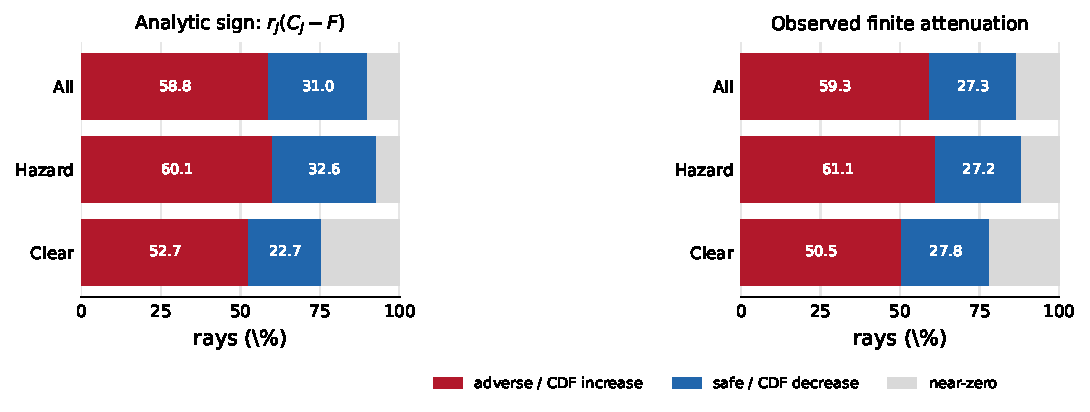
\includegraphics[width=\linewidth]{figures/v71_m49_attenuation_sign_boundary.pdf}
  \caption{M49 attenuation sign boundary on 99,208 frozen rays. Red denotes the analytically adverse direction (left)
  or an observed increase in the pre-boundary CDF (right); blue denotes the corresponding safe/decreasing direction.
  The result is descriptive and is never converted into a selection rule.}
  \label{fig:m49-sign-boundary}
\end{figure}

\begin{figure}[t]
  \centering
  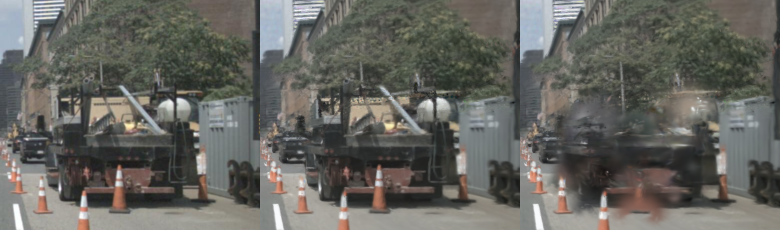
\includegraphics[width=\linewidth]{figures/v71_m24_geometry_locked_render.png}
  \caption{Frozen M24 view, cropped identically. Left to right: target image, original 32,522-primitive StreetGS Actor, and the 309-primitive geometry-locked carrier. Attribute transfer is rasterizer-compatible but loses appearance capacity; geometry is not moved to repair the image.}
  \label{fig:m24-render}
\end{figure}

\paragraph{Qualitative protocol.}
Main-paper and supplement scenes are frozen from metadata and registered failure strata before rendering method outputs. Panels show RGB, LiDAR, physical surface, ray evidence, compiler action, and the repaired world. We report all frozen cases, including failures, rather than selecting only visually favorable examples.
